\documentclass{article}



\usepackage{arxiv}

\usepackage[utf8]{inputenc} % allow utf-8 input
\usepackage[T1]{fontenc}    % use 8-bit T1 fonts
\usepackage{hyperref}       % hyperlinks
\usepackage{url}            % simple URL typesetting
\usepackage{booktabs}       % professional-quality tables
\usepackage{amsfonts}       % blackboard math symbols
\usepackage{nicefrac}       % compact symbols for 1/2, etc.
\usepackage{microtype}      % microtypography
\usepackage{lipsum}		% Can be removed after putting your text content
\usepackage{graphicx}
\usepackage[super]{natbib}
\usepackage{doi}
\usepackage{float}
\usepackage{amsmath}
\usepackage{mathrsfs}
\usepackage{caption} 
\usepackage{multicol}
\usepackage{pgfplots}
\usepackage{sectsty}
\usepackage{cancel}
\usepackage{amsmath}
\usepackage{amssymb}
\usepackage{listings}
\usepackage{algorithm}
\usepackage{algpseudocode}
\DeclareUnicodeCharacter{2212}{-}
\usetikzlibrary{patterns}
\usetikzlibrary{calc}
\usepackage{multirow}
\usepackage{outlines}
% \usepackage[table,xcdraw]{xcolor}
\usepackage{colortbl}


\title{\emph{Cryptologic Protocol Theory}}

\newcommand{\mycomment}[1]{}
\NewDocumentCommand{\codeword}{v}{%
\texttt{\textcolor{blue}{#1}}%
}


%\date{September 9, 1985}	% Here you can change the date presented in the paper title
%\date{} 					% Or removing it

\author{{\hspace{1mm}Rajat Dua} \\
	Master of Science - Computer Science\\
	Aarhus University\\
	\texttt{au747653@uni.au.dk / 202303549@post.au.dk} \\
	%% examples of more authors
	\And
	{\hspace{1mm}Jesper / Sophia} \\
	Institut for Datalogi\\
	Aarhus University\\
	%% \AND
	%% Coauthor \\
	%% Affiliation \\
	%% Address \\
	%% \texttt{email} \\
	%% \And
	%% Coauthor \\
	%% Affiliation \\
	%% Address \\
	%% \texttt{email} \\
	%% \And
	%% Coauthor \\
	%% Affiliation \\
	%% Address \\
	%% \texttt{email} \\
}

% Uncomment to remove the date
\date{February 7, 2024}

% Uncomment to override  the $A preprint' in the header
\renewcommand{\headeright}{Rajat Dua}
\renewcommand{\undertitle}{Week 2 - Zero Knowledge Proofs}
\renewcommand{\shorttitle}{\textit{Cryptology Protocol Theory} Notes}

%%% Add PDF metadata to help others organize their library
%%% Once the PDF is generated, you can check the metadata with
%%% $ pdfinfo template.pdf
\hypersetup{
pdftitle={Cryptology Protocol Theory Notes},
pdfsubject={q-bio.NC, q-bio.QM},
pdfauthor={Rajat Dua},
pdfkeywords={cryptology protocol theory, notes, au, aarhus, university},
}
\captionsetup[table]{skip=10pt}

% \subsectionfont{\underline}

\begin{document}
\maketitle
\vspace{-1cm}

\section{Introduction}

The requirement is that in between two parties, a prover and a verifier. Prover needs to prove that they really are who they are to the verifier. One can use passwords or secret key to tell the verifier that it is really them. Where the verifier has access to some public parameters to confirm if it is really them or not, such as hash of the password or public key. However, the issue is that you are revealing too much information which means someone can mimic as a prover.

This doesn't work in a real-world scenario. Let's think of another scheme where we introduce a challenge. 


\begin{figure}[h]
    \centering

\tikzset{every picture/.style={line width=0.75pt}} %set default line width to 0.75pt        

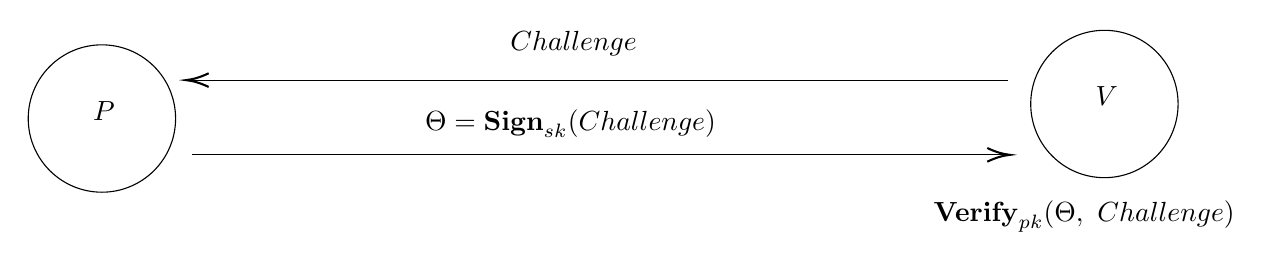
\begin{tikzpicture}[x=0.75pt,y=0.75pt,yscale=-1,xscale=1]
%uncomment if require: \path (0,300); %set diagram left start at 0, and has height of 300

%Shape: Circle [id:dp8041282073857139] 
\draw   (63,144.5) .. controls (63,124.89) and (78.89,109) .. (98.5,109) .. controls (118.11,109) and (134,124.89) .. (134,144.5) .. controls (134,164.11) and (118.11,180) .. (98.5,180) .. controls (78.89,180) and (63,164.11) .. (63,144.5) -- cycle ;
%Shape: Circle [id:dp437047467186648] 
\draw   (546,137.5) .. controls (546,117.89) and (561.89,102) .. (581.5,102) .. controls (601.11,102) and (617,117.89) .. (617,137.5) .. controls (617,157.11) and (601.11,173) .. (581.5,173) .. controls (561.89,173) and (546,157.11) .. (546,137.5) -- cycle ;
%Straight Lines [id:da8508776448739208] 
\draw    (535,126) -- (141,126) ;
\draw [shift={(139,126)}, rotate = 360] [color={rgb, 255:red, 0; green, 0; blue, 0 }  ][line width=0.75]    (10.93,-3.29) .. controls (6.95,-1.4) and (3.31,-0.3) .. (0,0) .. controls (3.31,0.3) and (6.95,1.4) .. (10.93,3.29)   ;
%Straight Lines [id:da617672878831609] 
\draw    (142,162) -- (534,162) ;
\draw [shift={(536,162)}, rotate = 180] [color={rgb, 255:red, 0; green, 0; blue, 0 }  ][line width=0.75]    (10.93,-3.29) .. controls (6.95,-1.4) and (3.31,-0.3) .. (0,0) .. controls (3.31,0.3) and (6.95,1.4) .. (10.93,3.29)   ;

% Text Node
\draw (93,135) node [anchor=north west][inner sep=0.75pt]   [align=left] {$\displaystyle P$};
% Text Node
\draw (576,128) node [anchor=north west][inner sep=0.75pt]   [align=left] {$\displaystyle V$};
% Text Node
\draw (294,101) node [anchor=north west][inner sep=0.75pt]   [align=left] {$\displaystyle Challenge$};
% Text Node
\draw (253,139) node [anchor=north west][inner sep=0.75pt]   [align=left] {$\displaystyle \Theta =\mathbf{Sign}_{sk}( Challenge)$};
% Text Node
\draw (498,183) node [anchor=north west][inner sep=0.75pt]   [align=left] {$\displaystyle \mathbf{Verify}_{pk}( \Theta ,\ Challenge)$};


\end{tikzpicture}
\end{figure}

\begin{align*}
    P \leftarrow V [Challenge] \\
    P \rightarrow V [\Theta = Sign_{sk}(Challenge)] \\
    V \rightarrow Verify_{pk}(\Theta, Challenge)
\end{align*}


We will later check man-in-the-middle attacks.

\begin{itemize}
    \item Good part: the prover can only create a signature with the secret key on the given challenge. [Convinces V]
    \item Bad part: the verifier can't be proved if they are malicious or not. [Revealing too much to V]
\end{itemize}

This was a signature scheme, however, we are still exposing a lot of information.

We want "Zero Knowledge". $V$ should learn nothing beyond the one bit we want them to learn.

\pagebreak

Let's take an encryption example instead of a signature one.

\begin{figure}[h]
    \centering
    

\tikzset{every picture/.style={line width=0.75pt}} %set default line width to 0.75pt        

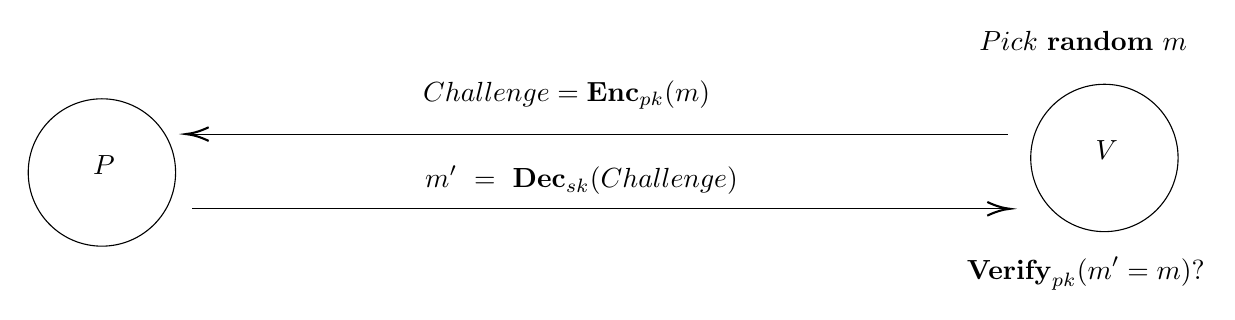
\begin{tikzpicture}[x=0.75pt,y=0.75pt,yscale=-1,xscale=1]
%uncomment if require: \path (0,300); %set diagram left start at 0, and has height of 300

%Shape: Circle [id:dp4801727704094567] 
\draw   (54,143.5) .. controls (54,123.89) and (69.89,108) .. (89.5,108) .. controls (109.11,108) and (125,123.89) .. (125,143.5) .. controls (125,163.11) and (109.11,179) .. (89.5,179) .. controls (69.89,179) and (54,163.11) .. (54,143.5) -- cycle ;
%Shape: Circle [id:dp4072819386380768] 
\draw   (537,136.5) .. controls (537,116.89) and (552.89,101) .. (572.5,101) .. controls (592.11,101) and (608,116.89) .. (608,136.5) .. controls (608,156.11) and (592.11,172) .. (572.5,172) .. controls (552.89,172) and (537,156.11) .. (537,136.5) -- cycle ;
%Straight Lines [id:da9083033772942881] 
\draw    (526,125) -- (132,125) ;
\draw [shift={(130,125)}, rotate = 360] [color={rgb, 255:red, 0; green, 0; blue, 0 }  ][line width=0.75]    (10.93,-3.29) .. controls (6.95,-1.4) and (3.31,-0.3) .. (0,0) .. controls (3.31,0.3) and (6.95,1.4) .. (10.93,3.29)   ;
%Straight Lines [id:da6134597201867293] 
\draw    (133,161) -- (525,161) ;
\draw [shift={(527,161)}, rotate = 180] [color={rgb, 255:red, 0; green, 0; blue, 0 }  ][line width=0.75]    (10.93,-3.29) .. controls (6.95,-1.4) and (3.31,-0.3) .. (0,0) .. controls (3.31,0.3) and (6.95,1.4) .. (10.93,3.29)   ;

% Text Node
\draw (84,134) node [anchor=north west][inner sep=0.75pt]   [align=left] {$\displaystyle P$};
% Text Node
\draw (567,127) node [anchor=north west][inner sep=0.75pt]   [align=left] {$\displaystyle V$};
% Text Node
\draw (243,98) node [anchor=north west][inner sep=0.75pt]   [align=left] {$\displaystyle Challenge=\mathbf{Enc}_{pk}( m)$};
% Text Node
\draw (244,139) node [anchor=north west][inner sep=0.75pt]   [align=left] {$\displaystyle m'\ =\ \mathbf{Dec}_{sk}( Challenge)$};
% Text Node
\draw (505,183) node [anchor=north west][inner sep=0.75pt]   [align=left] {$\displaystyle \mathbf{Verify}_{pk}( m'=m) ?$};
% Text Node
\draw (511,74) node [anchor=north west][inner sep=0.75pt]   [align=left] {$\displaystyle Pick\ \mathbf{random} \ m$};


\end{tikzpicture}

\end{figure}

\begin{align*}
    P \leftarrow V [Challenge, \in_{R} m, Challenge = Enc_{pk}(m)] \\
    P \rightarrow V [m' = Dec_{sk}(Challenge)] \\
    V \rightarrow Verify(m' = m)?
\end{align*}

\begin{itemize}
    \item Good part: Convinces $V$
    \item Bad part: Revealing too much information because we can use the ciphertext or challenge in such a way that this system becomes like a decryption oracle.
\end{itemize}

$m'$ is still too much information. So, we can use commitment ($\gamma$) to tackle the information revealed to an unwanted party.

\begin{figure}[h]
    \centering
    

\tikzset{every picture/.style={line width=0.75pt}} %set default line width to 0.75pt        

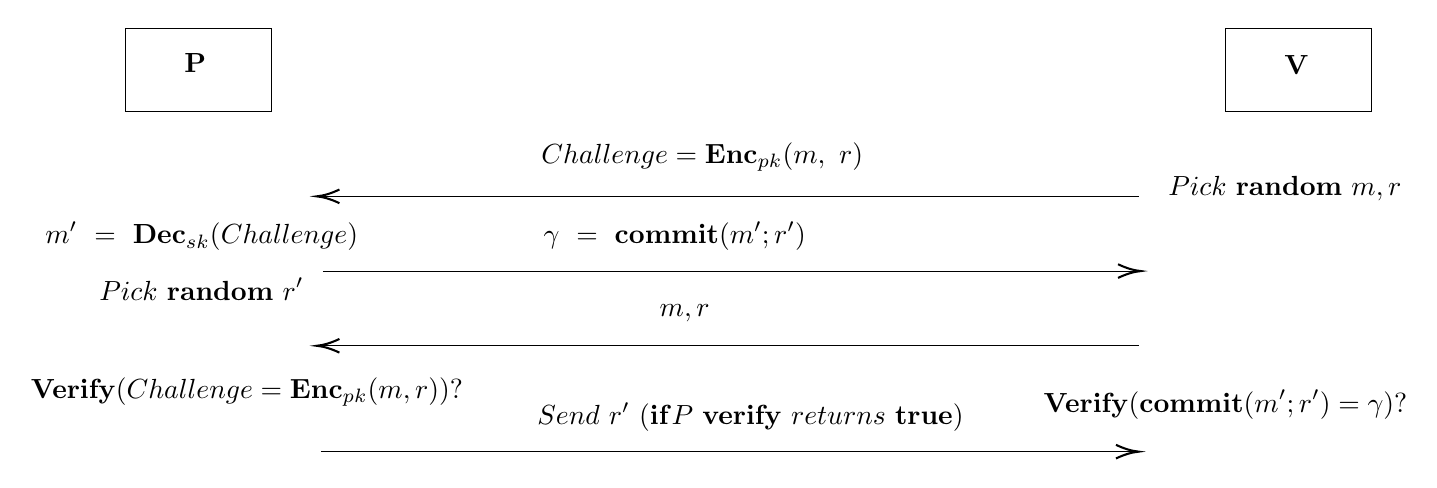
\begin{tikzpicture}[x=0.75pt,y=0.75pt,yscale=-1,xscale=1]
%uncomment if require: \path (0,300); %set diagram left start at 0, and has height of 300

%Straight Lines [id:da656306693676989] 
\draw    (537,94) -- (143,94) ;
\draw [shift={(141,94)}, rotate = 360] [color={rgb, 255:red, 0; green, 0; blue, 0 }  ][line width=0.75]    (10.93,-3.29) .. controls (6.95,-1.4) and (3.31,-0.3) .. (0,0) .. controls (3.31,0.3) and (6.95,1.4) .. (10.93,3.29)   ;
%Straight Lines [id:da3736965572998385] 
\draw    (144,130) -- (536,130) ;
\draw [shift={(538,130)}, rotate = 180] [color={rgb, 255:red, 0; green, 0; blue, 0 }  ][line width=0.75]    (10.93,-3.29) .. controls (6.95,-1.4) and (3.31,-0.3) .. (0,0) .. controls (3.31,0.3) and (6.95,1.4) .. (10.93,3.29)   ;
%Straight Lines [id:da8679256451189539] 
\draw    (537,166) -- (143,166) ;
\draw [shift={(141,166)}, rotate = 360] [color={rgb, 255:red, 0; green, 0; blue, 0 }  ][line width=0.75]    (10.93,-3.29) .. controls (6.95,-1.4) and (3.31,-0.3) .. (0,0) .. controls (3.31,0.3) and (6.95,1.4) .. (10.93,3.29)   ;
%Straight Lines [id:da8912568424702885] 
\draw    (143,217) -- (535,217) ;
\draw [shift={(537,217)}, rotate = 180] [color={rgb, 255:red, 0; green, 0; blue, 0 }  ][line width=0.75]    (10.93,-3.29) .. controls (6.95,-1.4) and (3.31,-0.3) .. (0,0) .. controls (3.31,0.3) and (6.95,1.4) .. (10.93,3.29)   ;
%Shape: Rectangle [id:dp9853812615092288] 
\draw   (49,13) -- (119,13) -- (119,53) -- (49,53) -- cycle ;
%Shape: Rectangle [id:dp6647756677531935] 
\draw   (579,13) -- (649,13) -- (649,53) -- (579,53) -- cycle ;

% Text Node
\draw (76,24) node [anchor=north west][inner sep=0.75pt]   [align=left] {$\displaystyle \mathbf{P}$};
% Text Node
\draw (606,25) node [anchor=north west][inner sep=0.75pt]   [align=left] {$\displaystyle \mathbf{V}$};
% Text Node
\draw (248,67) node [anchor=north west][inner sep=0.75pt]   [align=left] {$\displaystyle Challenge=\mathbf{Enc}_{pk}( m,\ r)$};
% Text Node
\draw (9,105) node [anchor=north west][inner sep=0.75pt]   [align=left] {$\displaystyle m'\ =\ \mathbf{Dec}_{sk}( Challenge)$};
% Text Node
\draw (490,186) node [anchor=north west][inner sep=0.75pt]   [align=left] {$\displaystyle \mathbf{Verify}(\mathbf{commit}( m';r') =\gamma ) ?$};
% Text Node
\draw (550,83) node [anchor=north west][inner sep=0.75pt]   [align=left] {$\displaystyle Pick\ \mathbf{random} \ m,r$};
% Text Node
\draw (249,105) node [anchor=north west][inner sep=0.75pt]   [align=left] {$\displaystyle \gamma \ =\ \mathbf{commit}( m';r')$};
% Text Node
\draw (35,132) node [anchor=north west][inner sep=0.75pt]   [align=left] {$\displaystyle Pick\ \mathbf{random} \ r'$};
% Text Node
\draw (305,145) node [anchor=north west][inner sep=0.75pt]   [align=left] {$\displaystyle m,r$};
% Text Node
\draw (2,180) node [anchor=north west][inner sep=0.75pt]   [align=left] {$\displaystyle \mathbf{Verify}( Challenge=\mathbf{Enc}_{pk}( m,r)) ?$};
% Text Node
\draw (246,192) node [anchor=north west][inner sep=0.75pt]   [align=left] {$\displaystyle Send\ r'\ (\mathbf{if} P\ \mathbf{verify} \ returns\ \mathbf{true})$};


\end{tikzpicture}

\end{figure}

\begin{align*}
    P \leftarrow V [Challenge, \in_{R} (m, r) | Challenge = Enc_{pk}(m;r)] \\
    P \rightarrow V [\gamma, m' = Dec_{sk}(c), r' \in_{R}  | \gamma = commit(m';r')] \\
    P \leftarrow V [m, r | P \rightarrow Verify(Challenge, Enc_{pk}(m;r))] \\
    P \rightarrow V [Execute \rightarrow Above_{True} | Send \: r'] \\
    V \rightarrow Verify(commit(m;r') = \gamma)?
\end{align*}

\begin{itemize}
    \item Convinces $V$
    \item Zero Knowledge
\end{itemize}

\section{Interactive Proof System}\label{week2-interactive-proof-system}

Let's define it more formally. For that, we call the interaction between prover and verifier as conversation which happens in a language. The goal is that prover is trying to prove to verifier an $x$ where the verifier either accepts or rejects it.

$$ P \rightarrow x \in \{0,1\}^* $$
$$ V \rightarrow x \in^{?} L \subset \{0,1\}^* $$

Language can be defined as palindrome, English but in this course, we will use \textbf{Graphs}. Mainly, isomorphic graphs are defined as follows:

$$L_{iso} = \{G_0, G_1 | \exists \text{ permutation } \pi \text{ such that } \pi(G_0) = G_1\}$$

$P, V, P*$ are turning machines ($P*$ is a cheating prover). We can say $(P,V)$ is an interactive proof system for $L$ if it provides following properties:

\begin{enumerate}
    \item (Efficiency) V is PPT
    \item (Completeness): If $x \in L, P_r[(P,V) \text{ rejects } x] = negl(|x|)$
    \item (Soundness): If $x \notin L, \forall P*, P_r[(P*,V) \text{ accepts } x] = negl(|x|)$
\end{enumerate}

Note: We don't want $P*$ to be PPT because $P*$ has infinite power and is trying to break this system. So, it makes this soundness definition more strong instead of saying a PPT $P$.

\subsection{Isomorphic Graphs}
A permutation on a graph means you can change the index of the vertex but not the direction of it. For example, let's create a graph between ($0, 1, \ldots, n$).

\begin{figure}[h]
    \centering
    

\tikzset{every picture/.style={line width=0.75pt}} %set default line width to 0.75pt        

\begin{tikzpicture}[x=0.75pt,y=0.75pt,yscale=-1,xscale=1]
%uncomment if require: \path (0,300); %set diagram left start at 0, and has height of 300


% Text Node
\draw (178,59) node [anchor=north west][inner sep=0.75pt]  [font=\Large] [align=left] {$\displaystyle 0$};
% Text Node
\draw (390,61) node [anchor=north west][inner sep=0.75pt]  [font=\Large] [align=left] {$\displaystyle 1$};
% Text Node
\draw (260,178) node [anchor=north west][inner sep=0.75pt]  [font=\Large] [align=left] {$\displaystyle n$};
% Connection
\draw    (195,73.09) -- (385,74.89) ;
\draw [shift={(387,74.91)}, rotate = 180.54] [color={rgb, 255:red, 0; green, 0; blue, 0 }  ][line width=0.75]    (10.93,-3.29) .. controls (6.95,-1.4) and (3.31,-0.3) .. (0,0) .. controls (3.31,0.3) and (6.95,1.4) .. (10.93,3.29)   ;
% Connection
\draw    (387,84.07) -- (280.48,180.68) ;
\draw [shift={(279,182.02)}, rotate = 317.79] [color={rgb, 255:red, 0; green, 0; blue, 0 }  ][line width=0.75]    (10.93,-3.29) .. controls (6.95,-1.4) and (3.31,-0.3) .. (0,0) .. controls (3.31,0.3) and (6.95,1.4) .. (10.93,3.29)   ;

\end{tikzpicture}
\end{figure}

So, a table for vertexes can be represented as:

\begin{table}[h]
\centering
\begin{tabular}{|l|l|l|l|l|}
\hline
\multicolumn{1}{|c|}{\textbf{Vertexes}} &
  \multicolumn{1}{c|}{\textbf{0}} &
  \multicolumn{1}{c|}{\textbf{1}} &
  \ldots &
  \multicolumn{1}{c|}{\textbf{n}} \\ \hline
\textbf{0} & \cellcolor[HTML]{C0C0C0} & \cellcolor[HTML]{C0C0C0} & \cellcolor[HTML]{FFCCC9} & \cellcolor[HTML]{C0C0C0} \\ \hline
\textbf{1} &
  1 &
  \cellcolor[HTML]{C0C0C0} &
  \cellcolor[HTML]{FFCCC9}{\color[HTML]{C0C0C0} } &
  \cellcolor[HTML]{C0C0C0}{\color[HTML]{C0C0C0} } \\ \hline
\vdots      & \cellcolor[HTML]{FFCCC9} & \cellcolor[HTML]{FFCCC9} & \cellcolor[HTML]{FFCCC9} & \cellcolor[HTML]{FFCCC9} \\ \hline
\textbf{n} & 0                        & 1                        & \cellcolor[HTML]{FFCCC9} & \cellcolor[HTML]{C0C0C0} \\ \hline
\end{tabular}
\end{table}

If one has to implement premutation, the max they can do is switch the labels of $0$ and $1$ but the edge remains in the same place.

\section{Interactive Argument System}

The same thing as above holds, however, there is an extra security feature with Prover ($P$) called a witness ($w$). Now, we need to satisfy the same conditions as above - 

\begin{enumerate}
    \item (Efficiency) $P,V$ are PPT
    \item (Completeness): If $x \in L, \exists \: w, P_r[(P(w),V) \text{ rejects } x] = negl(|x|)$
    \item (Soundness): If $x \notin L, \forall \text{ PPT } P*, P_r[(P*,V) \text{ accepts } x] = negl(|x|)$
\end{enumerate}

\section{Interactive Zero Knowledge Proof}

Let's call a conversation between an actual prover ($P$) and verifier ($V$) as $\mathcal{T}_{R}$ called "Real Transcript". We want to build a simulator that will try to mimic this real conversation however this simulator ($S$) doesn't have access to infinite power or access to the witness ($w$). Let's call the conversation for the simulator as $\mathcal{T}_{S}$ which is called "Simulated Transcript".

The proof says that $$\mathcal{T}_{S} \thicksim \mathcal{T}_{R}$$

Now, $\thicksim$ is indistinguishable. This holds for all: Unconditional, Statistical and Computational.

So, if the simulator doesn't have access to the above things, how can they try to simulate a real transcript? \textbf{Reason}: maybe the simulator can change the order in such a way that they can use the second message first which can provide "more" advantage.

\subsection{Formal Definition - Honest Verifier}

It states that $\exists$ PPT $S$ such that $\forall \: x \in L, \mathcal{T}_{R} \thicksim \mathcal{T}_{S} = S(x)$

However, this isn't strong enough since a verifier can be dishonest.

\subsection{Formal Definition - All Verifier}

It states that $\forall$ PPT $V*, \exists \: S_{V*} | \forall \: x \in L, \mathcal{T}_{R} \thicksim \mathcal{T}_{S_{V*}}$

Here the $\mathcal{T}_{R}$ can either be the actual conversation or a corrupted one. It is not the same $\mathcal{T}_{R}$ as an honest verifier since we are working with "all" kinds of verifiers.

\subsection{Isomorphic Graphs (Cont.)}

There is a conversation between a prover and a verifier. Where $x = (G_0, G_1)$, where these groups are isomorphic in the same class. Prover selects a witness ($w = \pi$) such that $\pi$ acts like a medium that satisfies the condition $G_1 = \pi(G_0)$. Note: $\pi$ is a permutation. You can go through the main section where isomorphic definition was mentioned here (\ref{week2-interactive-proof-system}).

The conundrum is that you cannot find $\pi$ for $(G_0, G_1)$ there is not algorithm for it. So, $V$ cannot compute it in PPT. 

\section{Approaches for ZKP}

\begin{enumerate}
    \item Commit $b$, do not open until $V$ proves knowledge of what you will open to. [Maybe if $V$ tells you the commit $b$ [Not sure]]
    \item Divide $w$ into two parts, such that both together can reveal $w$. However, each alone does not tell you about anything. Moreover, it needs to be "verifiable". [We do not know how to break $w$ yet]
\end{enumerate}


% \bibliographystyle{unsrtnat}
% \bibliography{references}

\end{document}
